% Preamble:
% \usepackage{tikz}
% \usepackage{xcolor}

\begin{figure}[ht]
\centering
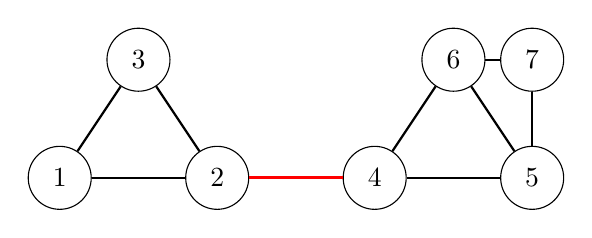
\begin{tikzpicture}[
  v/.style={circle, draw, minimum size=8mm},
  e/.style={thick},
  bridge/.style={very thick, red}
]

% --- vertices ---
\node[v] (1) at (0,0)   {$1$};
\node[v] (2) at (2,0)   {$2$};
\node[v] (3) at (1,1.5) {$3$};

\node[v] (4) at (4,0)   {$4$};
\node[v] (5) at (6,0)   {$5$};
\node[v] (6) at (5,1.5) {$6$};
\node[v] (7) at (6,1.5) {$7$};

% --- edges (connected graph) ---
% left triangle
\draw[e] (1)--(2);
\draw[e] (2)--(3);
\draw[e] (3)--(1);

% right cluster
\draw[e] (4)--(5);
\draw[e] (4)--(6);
\draw[e] (5)--(6);
\draw[e] (6)--(7);
\draw[e] (5)--(7);

% bridge edge (removing it disconnects the graph)
\draw[bridge] (2)--(4);

\end{tikzpicture}
\caption{A connected undirected graph on 7 vertices. The red edge $(2,4)$ is a \emph{bridge}: removing it disconnects the graph into two components (the triangle on $\{1,2,3\}$ and the subgraph on $\{4,5,6,7\}$).}
\label{fig:bridge-example}
\end{figure}
